%%%%%%%%%%%%%%%%%%%%%%%%%%%%%%%%%%%%%%%%%
% Journal Article
% LaTeX Template
% Version 1.4 (15/5/16)
%
% This template has been downloaded from:
% http://www.LaTeXTemplates.com
%
% Original author:
% Frits Wenneker (http://www.howtotex.com) with extensive modifications by
% Vel (vel@LaTeXTemplates.com)
%
% License:
% CC BY-NC-SA 3.0 (http://creativecommons.org/licenses/by-nc-sa/3.0/)
%
%%%%%%%%%%%%%%%%%%%%%%%%%%%%%%%%%%%%%%%%%

%----------------------------------------------------------------------------------------
%	PACKAGES AND OTHER DOCUMENT CONFIGURATIONS
%----------------------------------------------------------------------------------------

\documentclass[10pt]{article} % Single column

%\documentclass[twoside,twocolumn]{article} % Two column

\usepackage{blindtext} % Package to generate dummy text throughout this template 

\usepackage[sc]{mathpazo} % Use the Palatino font
\usepackage[T1]{fontenc} % Use 8-bit encoding that has 256 glyphs
\linespread{1.05} % Line spacing - Palatino needs more space between lines
\usepackage{microtype} % Slightly tweak font spacing for aesthetics

\usepackage[spanish]{babel} % Language hyphenation and typographical rules

\usepackage[hmarginratio=1:1,top=32mm,columnsep=20pt]{geometry} % Document margins
\usepackage[hang, small,labelfont=bf,up,textfont=it,up]{caption} % Custom captions under/above floats in tables or figures
\usepackage{booktabs} % Horizontal rules in tables

\usepackage{lettrine} % The lettrine is the first enlarged letter at the beginning of the text

\usepackage{enumitem} % Customized lists
\setlist[itemize]{noitemsep} % Make itemize lists more compact

\usepackage{abstract} % Allows abstract customization
\renewcommand{\abstractnamefont}{\normalfont\bfseries} % Set the "Abstract" text to bold
\renewcommand{\abstracttextfont}{\normalfont\small\itshape} % Set the abstract itself to small italic text

\usepackage{titlesec} % Allows customization of titles
\renewcommand\thesection{\Roman{section}} % Roman numerals for the sections
\renewcommand\thesubsection{\roman{subsection}} % roman numerals for subsections
\titleformat{\section}[block]{\large\scshape\centering}{\thesection.}{1em}{} % Change the look of the section titles
\titleformat{\subsection}[block]{\large}{\thesubsection.}{1em}{} % Change the look of the section titles

\usepackage{fancyhdr} % Headers and footers
\pagestyle{fancy} % All pages have headers and footers
\fancyhead{} % Blank out the default header
\fancyfoot{} % Blank out the default footer
\fancyhead[C]{Lenguajes de Programaci\'on: \textbf{Python M\'agico}} % Custom header text
\fancyfoot[RO,LE]{\thepage} % Custom footer text

\usepackage{titling} % Customizing the title section

\usepackage{hyperref} % For hyperlinks in the PDF

\usepackage{graphicx} % For images

\usepackage{pifont} % bullets

% Keywords command
\providecommand{\keywords}[1]
{
	\small	
	\vspace{0.5em}
	\noindent \textbf{\textit{Palabras clave --- }} #1
}


%----------------------------------------------------------------------------------------
%	TITLE SECTION
%----------------------------------------------------------------------------------------

\setlength{\droptitle}{-4\baselineskip} % Move the title up

\pretitle{\begin{center}\Huge\bfseries} % Article title formatting
\posttitle{\end{center}} % Article title closing formatting
\title{\normalsize{Lenguajes de Programaci\'on}\\
\Huge\bfseries Python M\'agico\\

\includegraphics[height=5em]{magic_logo.png}} % Article title
\author{% 
\normalsize\textsc{Leandro Rodr\'iquez Llosa}\\
\normalsize\textsc{Laura V. Riera P\'erez}\\ 
\normalsize\textsc{Marcos M. Tirador del Riego} \\[2ex]
\small Tercer a\~no. Ciencias de la Computaci\'on. \\ % institution
\small Facultad de Matem\'atica y Computaci\'on, Universidad de La Habana, Cuba \\ % institution
}
\date{\footnotesize Noviembre 2022 } % Leave empty to omit a date


% Abstract configurations
\renewenvironment{abstract}
{\small
	\begin{center}
		\bfseries \abstractname\vspace{-.5em}\vspace{0pt}
	\end{center}
	\list{}{
		\setlength{\leftmargin}{1.5cm}%
		\setlength{\rightmargin}{\leftmargin}%
	}%
	\item\relax}
{\endlist}


\usepackage{todonotes} % \TODO
\usepackage{listings} % Code listings
\usepackage{xcolor}
\definecolor{backcolour}{rgb}{0.95,0.95,0.92}

\newcommand{\csl}[1]{\colorbox{backcolour}{\texttt{#1}}}

\newcommand{\imgcaption}[2]{\tiny \textbf{Figura #1.} #2.}

\newcommand{\mgc}[2][]{\colorbox{backcolour}{\texttt{\_\_#2\_\_#1}}}

% Hyperlinks configurations
\hypersetup{
	colorlinks=true,
	linkcolor=black,
	filecolor=magenta,      
	urlcolor=cyan,
	pdftitle={Overleaf Example},
	pdfpagemode=FullScreen,
}

%----------------------------------------------------------------------------------------

\begin{document}
% Print the title
\maketitle

% ABSTRACT
\begin{abstract}
	\noindent \blindtext % Dummy abstract text - replace \blindtext with your abstract text
	
	\keywords{Palabra 1 \textbf{$\cdot$} Palabra 2 \textbf{$\cdot$} Palabra 3}
\end{abstract}


%----------------------------------------------------------------------------------------
%	ARTICLE CONTENTS
%----------------------------------------------------------------------------------------

\vspace{1em}
\section{M\'etodos M\'agicos}

Los m\'etodos m\'agicos son un conjunto de m\'etodos especiales en Python, cuyo nombre comienza y termina con dos guiones bajos. Lo que hace especiales o ``m\'agicos'' a estos m\'etodos es que no tienen que ser invocados directamente, sino que la invocaci\'on ocurre internamente desde la clase, bajo una determinada acci\'on. Estos m\'etodos tambi\'en son llamados dunder, que es una abreviatura de ``Double Underscore'', que significa doble gui\'on bajo en ingl\'es. 

En este seminario se ver\'a el uso de alguno de los m\'etodos m\'agicos m\'as importantes. Para ello se implementar\'a una clase \emph{Matrix} para representar matrices, con algunas funcionalidades b\'asicas.

Se comenzar\'a hablando del m\'etodo \mgc{init}. Este m\'etodo es invocado cuando se crea una instancia de una clase. Este act\'ua como un constructor cuya funci\'on es inicializar las propiedades de la clase. Es por esto que el programador, para lograr el comportamiento deseado en la instanciaci\'on de una clase definida por \'el, debe redefinir el cuerpo de este m\'etodo en la clase.

Sin embargo, es bueno saber que cuando uno instancia una clase, \mgc{init} no es el primer m\'etodo m\'agico que es invocado. Antes es llamado el m\'etodo  \mgc{new}. Este m\'etodo es el responsable de crear la instancia de la clase y luego se la pasa al m\'etodo \mgc{init} junto con los argumentos. Explicar la utilidad de esta clase se sale del prop\'osito de este seminario.

Se puede observar en la implementaci\'on siguiente del constructor de la clase Matrix.

\begin{center}
	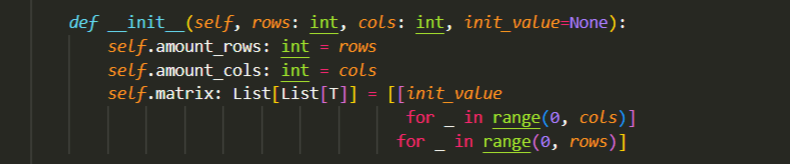
\includegraphics[width=12cm]{init.png}
	
	\imgcaption{1}{Constructor de la clase Matrix}
\end{center}


\subsection{Operadores}

Una de las ventajas de usar los m\'etodos  m\'agicos en Python es que permiten realizar operaciones con los objetos definidos como si fueran built-in. Por ejemplo si se quisiera saber si dos objetos son iguales habr\'ia que crear en la clase alg\'un tipo de m\'etodo \csl{equals} que permita definir el comportamiento de la comparaci\'on entre dos instancias de la clase. Pero Python simplifica este comportamiento al permitirte redefinir el m\'etodo m\'agico \mgc[()]{eq}. De esta forma podemos comparar dos objetos de un mismo tipo simplemente haciendo uso del operador \csl{==}. Si no redefinimos este m\'etodo en nuestra clase el comportamiento por defecto es que da un resultado positivo si y solo si las instancias de la clase que se est\'an comparando son exactamente la misma.

Se presenta el c\'odigo empleado para definir en la clase Matrix la posibilidad de comparar dos matrices solamente usando \csl{==}.

\begin{center}
	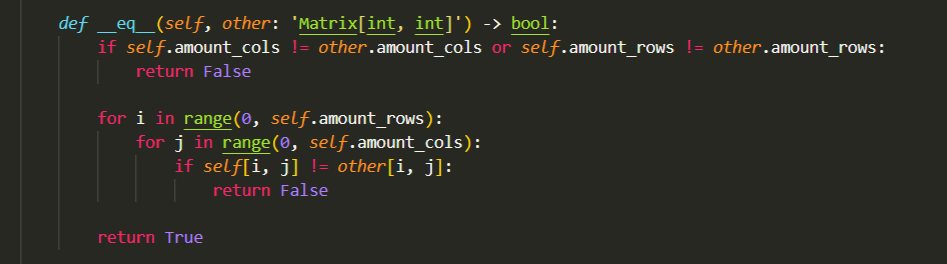
\includegraphics[width=14cm]{eq.png} 
	
	\imgcaption{2}{Operador igual}
\end{center}


N\'otese como al hacer uso de los m\'etodos dunder el programador se ahorra tener que definir m\'etodos propios para imitar el comportamiento de operaciones b\'asicas. Adem\'as el llamado a estos m\'etodos que se habr\'ian de crear, ser\'ia engorroso y menos natural. Casi todos los operadores significativos pueden ser redefinidos a trav\'es de su m\'etodo m\'agico correspondiente. Se mostrar\'an a continuaci\'on dos operadores aritm\'eticos b\'asicos que fueron redefinidos en la clase Matrix. Estos son la suma, a partir de \mgc{add} y la multiplicaci\'on a partir de \mgc{mul}.

\begin{center}
	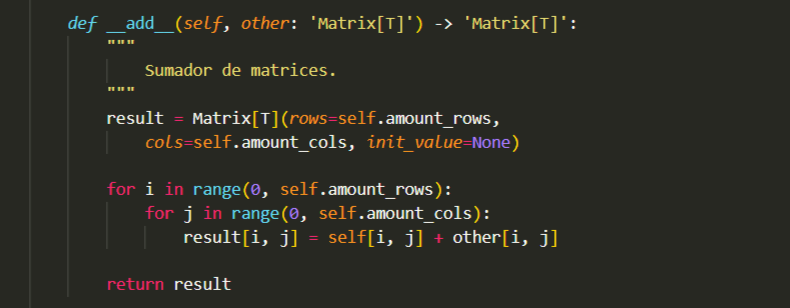
\includegraphics[width=12cm]{add.png} 
	
	\imgcaption{3}{Operador suma}
\end{center}

\begin{center}
	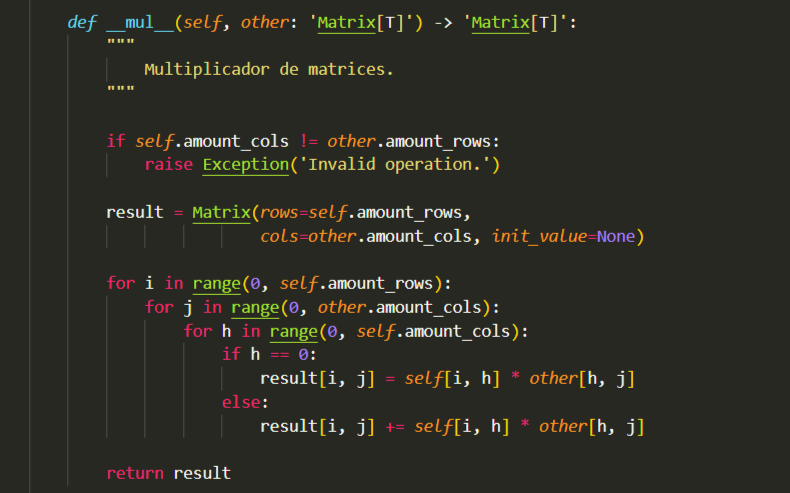
\includegraphics[width=12cm]{mul.png}
	
	\imgcaption{4}{Operador multiplicaci\'on}
\end{center}

\subsection{Indexaci\'on}
Los m\'etodos m\'agicos en Python tambi\'en permiten a\~nadir la funcionalidad de indexar mediante corchetes para acceder al valor de un elemento, tanto para leer el mismo al redefinir \mgc{getitem} o modificarlo al redefinir \mgc{setitem}. Estos m\'etodos se invocan automáticamente cuando se usa el operador indexador \csl{[ ]} con la variable de referencia de la clase. Para secuencias, los \'indices aceptados deben ser números enteros y slices. La interpretación especial de los índices negativos depende de la redefinici\'on método. Si el \'indice es de un tipo inapropiado, se puede generar \csl{TypeError}, y si tiene un valor fuera del conjunto de índices de la secuencia, debe generarse \csl{IndexError}. Para los tipos de asignación, si falta el \'indice, se debe generar \csl{KeyError}.

A continuaci\'on se muestra la implementaci\'on dada a ambos, 
\mgc{getitem} y \mgc{setitem}, al redefinirlos en la clase Matrix:

\begin{center}
	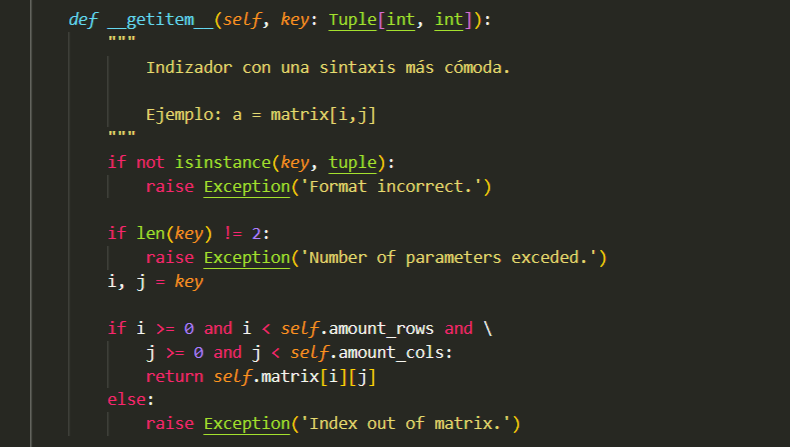
\includegraphics[width=12cm]{getitem.png}
	
	\imgcaption{5}{Indexaci\'on para obtener el valor de un elemento de la matriz}
\end{center}

\begin{center}
	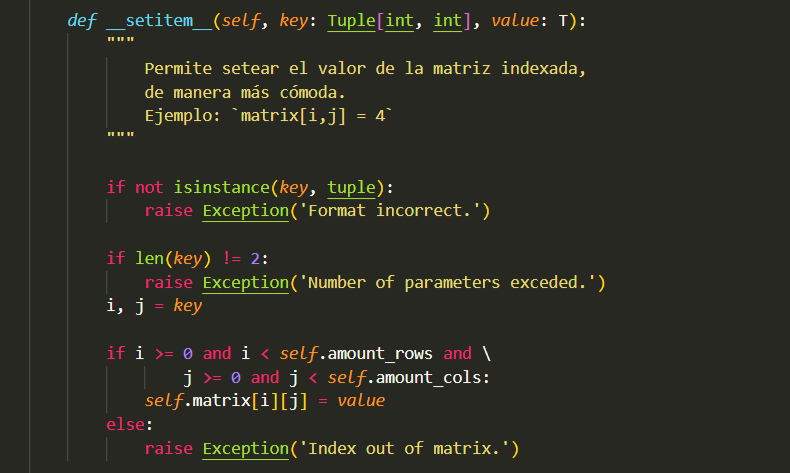
\includegraphics[width=12cm]{setitem.png}
	
	\imgcaption{6}{Indexaci\'on para asignar un nuevo valor a un elemento de la matriz}
\end{center}

\subsection{Iteraci\'on}

\mgc{next}

\begin{center}
	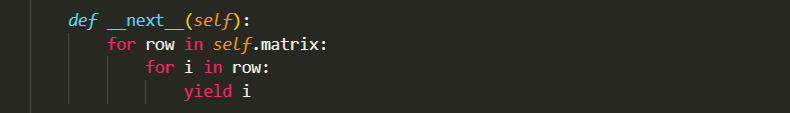
\includegraphics[width=12cm]{next.png}
	
	\imgcaption{7}{Operador multiplicaci\'on}
\end{center}


\mgc{iter}

\begin{center}
	
\includegraphics[width=12cm]{iter.png}
	
	\imgcaption{8}{Operador multiplicaci\'on}
\end{center}

\subsection{Atributos}

A trav\'es del uso de los m\'etodos m\'agicos Python permite controlar el acceso a los atributos de una clase. Esto es, permite definir un comportamiento determinado cuando se intente acceder a un atributo de la clase, incluso cuando este atributo no existe. Esto nos da la posibilidad, por ejemplo, de prohibir el acceso a ciertos atributos de la clase. Incluso da la posibilidad de modificar los atributos de la clase en tiempo de compilaci\'on. \todo{revisar la validez de la oracion anterior pues no estoy seguro al 100}. Se ver\'an a continuaci\'on 3  m\'etodos que permiten este comportamiento.

\begin{itemize}
	\item \mgc{getattribute} Este m\'etodo es lo primero que se invoca cuando se intenta acceder a un atributo de una clase, sin importar si este existe o no. Permite definir reglas de comportamiento en respuesta al acceso al atributo. El comportamiento del m\'etodo por defecto es buscar si el atributo existe, retornando su valor en caso afirmativo y lanzando \csl{AttributeError} en caso contrario.
	\item \mgc{getattr} Este m\'etodo es invocado siempre que se intente acceder a un atributo que no existe en un objeto. Adem\'as, si el m\'etodo anterior lanza \csl{AttributeError} desp\'ues de su ejecuci\'on, esta excepci\'on es ignorada y este m\'etodo es invocado. 
	\item \mgc{setattr} Similar al primero de estos tres, este m\'etodo siempre es invocado cuando se intenta cambiar el valor de un atributo. De igual forma su uso suele ser aplicar algunas reglas antes de que se ejecute la modificaci\'on. Adicionalmente puede usarse para definir un comportamiento si el atributo en cuesti\'on no existe.
\end{itemize}

Hay que tener cierto cuidado al usar estos tres m\'etodos. Sucede que si en el cuerpo del m\'etodo se hace uso de alg\'un otro atributo de la clase, entonces el m\'etodo ser\'a invocado nuevamente provocando una recursi\'on infinita.

A continuaci\'on se presenta la forma en que se redefinieron los m\'etodos \mgc{getattr} y \mgc{setattr} en la clase Matrix.

\begin{center}
	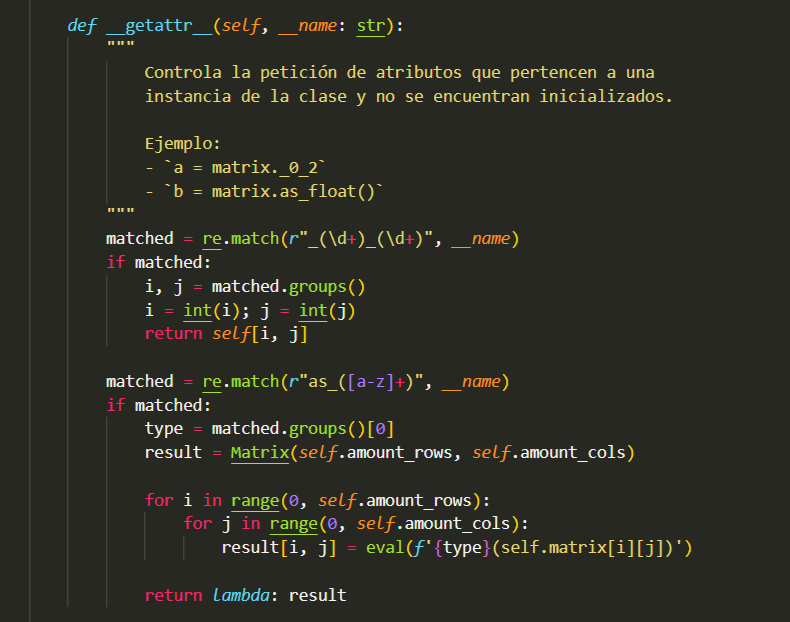
\includegraphics[width=12cm]{getattr.png} 
	
	\imgcaption{9}{Constructor de la clase Matrix}
\end{center}

\begin{center}
	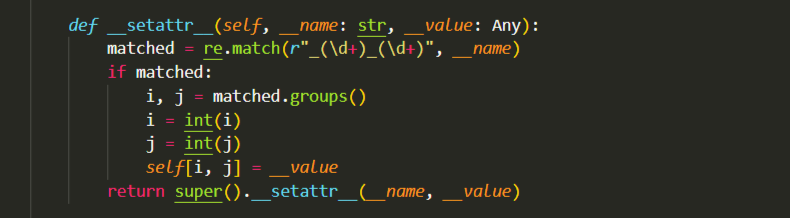
\includegraphics[width=12cm]{setattr.png}
	
	\imgcaption{10}{Constructor de la clase Matrix}
\end{center}

Una de las ideas con el uso del \mgc{setattr} y \mgc{getattr} es poder indexar en la matriz $m$ usando la forma \csl{$m.\_i\_j$} donde $i$ y $j$ son los \'indices a los que se quiere acceder. Como \csl{$\_i\_i$} no es un atributo de Matrix, al intentar acceder al valor del mismo el programa invoca al m\'etodo \mgc{getattr} despu\'es de ejecutar \mgc{getattribute} sin \'exito. Entonces al m\'etodo en cuesti\'on es pasado como par\'ametro el nombre del atributo al que se quiere acceder. Haciendo uso de la biblioteca \csl{re} para comprobar patrones en expresiones regulares, podemos comparar el nombre del m\'etodo con el patr\'on \csl{$\_i\_j$}, y si coinciden solamente debemos obtener los enteros $i$ y $j$ del nombre, y devolver \csl{$self[i][j]$}. An\'alogamente se hace con \mgc{setattr} pero esta vez para modificar el valor en esa posici\'on. La diferencia es que como se explicaba antes, este m\'etodo se llama independientemente de si el atributo aparece o no, pero en este caso de igual modo este atributo no existe.

N\'otese que la idea usada anteriormente consisti\'o en poder invocar un comportamiento determinado, como si fuera un atributo de la clase. Una idea similar usamos para lograr castear el tipo de los elementos en la matriz representada por la clase Matrix, a otro tipo diferente. Se quiere que este comportamiento se pueda lograr de la forma \csl{m.as\_type()} (por ejemplo se pudiera llamar a \csl{m.as\_float()} para obtener una nueva matriz con todos sus valores de tipo float). Pero se puede adicionar otro comportamiento al m\'etodo \mgc{getattr}, ya que Matrix no contiene un atributo \csl{as\_type} para ninguna cadena ``tpye''. La idea es de modo similar, haciendo uso de \csl{re}, reconocer el patr\'on de \csl{as\_type} en el nombre del atributo. Si este coincide se crea una matriz nueva del tipo en cuesti\'on y se castea cada elemento de la matriz anterior al tipo nuevo. Para esto \'ultimo se hace uso del m\'etodo \csl{eval} que eval\'ua el texto de un string como si fuera una sentencia de c\'odigo python. Finalmente se devuelve como resultado de la invocaci\'on de este m\'etodo, una expresi\'on lambda cuyo cuerpo consiste solamente de retornar la nueva matriz. Esto se hace ya que la sentencia \csl{m.as\_type()} espera que el atributo \csl{as\_type} devuelva una funci\'on, que se invocar\'a inmediatamente sin argumentos.

\subsection{Otros m\'etodos utilizados}

\colorbox{backcolour}{\mgc{repr}}

\begin{center}
	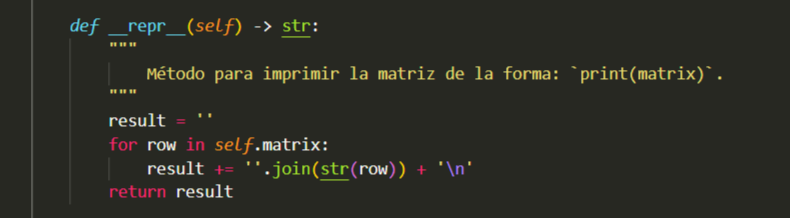
\includegraphics[width=12cm]{repr.png}
	
	\imgcaption{11}{Constructor de la clase Matrix}
\end{center}

\colorbox{backcolour}{\mgc{len}}

\begin{center}
	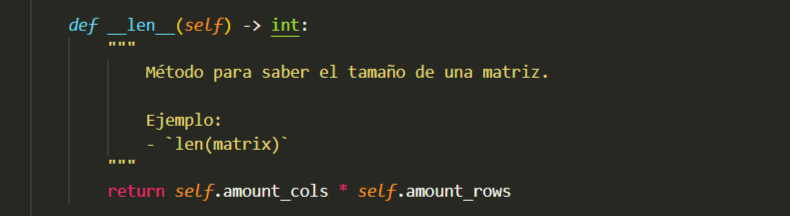
\includegraphics[width=12cm]{len.png}
	
	\imgcaption{12}{Constructor de la clase Matrix}
\end{center}

\colorbox{backcolour}{\mgc{call}}

\begin{center}
	
\includegraphics[width=12cm]{call.png}
	
	\imgcaption{13}{Constructor de la clase Matrix}
\end{center}

%----------------------------------------------------------------------------------------
%	REFERENCE LIST
%----------------------------------------------------------------------------------------

\begin{thebibliography}{99} % Bibliography - this is intentionally simple in this template

\bibitem[Figueredo and Wolf, 2009]{Figueredo:2009dg}
Figueredo, A.~J. and Wolf, P. S.~A. (2009).
\newblock Assortative pairing and life history strategy - a cross-cultural
  study.
\newblock {\em Human Nature}, 20:317--330.
 
\end{thebibliography}

%----------------------------------------------------------------------------------------

\end{document}
